\newtheorem{theorem}{Theorem.}
\newcommand{\hot}[0]{h.o.t}
%WARNING: amsmath not available


This chapter describes the \cgal's package geared towards the
estimation of local differential quantities on sampled surfaces, known
either as a mesh or a point cloud.
 
%%%%%%%%%%%%%%%%%%%%%%%
\section{Introduction}
\label{sec:intro}
%%%%%%%%%%%%%%%%%%%%%%%

\subsection{Overview}
%%%%%%%%%%%%%%%%%%%%%%

Consider a sampled smooth surface, and assume we are given a
collection of points $P$ about a given sample $p$. We aim at
estimating the differential properties up to any fixed order of the
surface at point $p$ from the point set $P^+ = P\cup \{ p\}$ ---we
denote $N=\mid P^+\mid$. More precisely, first order properties
correspond to the normal or the tangent plane; second order properties
provide the principal curvatures and directions, third order
properties provide the directional derivatives of the principal
curvatures along the curvature lines, etc.  Most of the time,
estimating first and second order differential quantities is
sufficient.  However, some applications involving shape analysis
require estimating third and fourth order differential quantities.
%%
Many different estimators have been proposed in the vast literature of
applied geometry \cite{cgal:p-smrqt-01}, and all of them need to
define a neighborhood around the point at which the estimation is
computed. These methods may be classified into two groups. The first
one features methods geared towards meshes
\cite{cgal:pp-cdmsc-93,cgal:mdsb-ddgot-02,cgal:csm-rdtnc-03}.
Such methods exploit the geometry and the topology of the mesh, and
are sometimes referred to as methods from {\em discrete differential
geometry}.
%%
The second one comprises methods relying on smooth differential
geometry calculations, carried out on smooth objects {\em fitted} from
the sample points provided. Such naturally accommodate meshes, but also
point clouds.

%On the other hand, fitting methods rely on smooth differential
%geometry and approximation, and hence are able to process point clouds
%directly.

%and use at different level the geometry of the mesh. On one hand,
%methods relying on {\em discrete differential geometry} only use the
%information provided by the mesh

%By now, there are two methods to extract local differential properties
%coming with theoretical analysis of their convergence rates. 


Estimating differential quantities naturally subsumes (i)\ a smooth
surface exists (ii)\ one wishes to recover its differential
properties. This two observations call for the convergence analysis of
the methods developed, and by now, two estimation methods come with
approximation guarantees measuring the convergence rate of the
discrepancy between the estimates and the true (unknown) values.

On one hand, the normal cycle theory is used in
\cite{cgal:csm-rdtnc-03} to provide an estimate of the  integral of the
$3D$ embedding \footnote{Recall that the Weingarten map is a bilinear
form of the tangent space, so that integrating it requires embedding
it in $3D$ since the tangent plane rotates.} of the Weingarten map of
surface discretized by a mesh.  On the other hand,
\cite{cgal:cp-edqpf-05} uses polynomial fitting to extract the
coefficients of the local representation of the surface as a height
function. The former method provides spatial averages, and is
particularly well suited to meshes. Yet, it is limited to second order
differential properties.
%%
The later one carries three advantages~: first, differential
properties of any order can be retrieved; second, the convergence
rates provided are the best ones known so far ---they are actually
optimal; third, point clouds can be directly handled ---no topological
information is required.


\subsection{Jets, Monge form and polynomial fitting}
%%%%%%%%%%%%%%%%%%%%%%%%%%%%%%%%

\paragraph{Smooth surfaces, $d$-jets and the Monge form.}
%
To present the method, we shall need the following notions. Consider a
smooth surface.  About one of its points, consider a coordinate system
whose $z$-axis does not belong to the tangent space. In such a frame,
the surface can locally be written as the graph of a bivariate
function. Denoting h $\hot$ standing for {\em higher order terms}, one
has~:
%
%Assume the surface is given, locally and in a suitable , as a height
%function ---with $\hot$ standing for {\em higher order terms}~:
\begin{equation}
z(x,y)=J_{B,d}(x,y) + \hot \ ; \quad 
J_{B,d}(x,y)=\sum_{k=0}^{k=d}(\sum_{i=0}^{i=k}
\frac{B_{k-i,i}x^{k-i}y^{i}}{i!(k-i)!}).
\end{equation}
The degree $d$ polynomial $J_{B,d}$ is the Taylor expansion of the
function $z$, an is called its $d$-jet. Notice that a $d$-jet contains
$N_d=(d+1)(d+2)/2$ coefficients.

Recall that an umbilical point of a surface ---or umbilic for short,
is a point where both principal curvatures are identical.  At any
point of the surface which is not an umbilic, principal directions
$d_1, d_2$ are well defined, and these (non oriented) directions
together with the normal vector $n$ define two direct orthonormal
frames. If $v_1$ is a unit vector of direction $d_1$ then there exists
a unique unit vector $v_2$ so that $(v_1,v_2,n)$ is direct; and the
other possible frame is $(-v_1,-v_2,n)$. In one of these Monge
coordinate systems, the surface is said to be given in the Monge form
and its jet has the following canonical form~:

\begin{eqnarray}
\label{eq:monge}
z(x,y) =  & \frac{1}{2}(k_1x^2 + k_2y^2)+
	\frac{1}{6}(b_0x^3+3b_1x^2y+3b_2xy^2+b_3y^3) \\
  &  +\frac{1}{24}(c_0x^4+4c_1x^3y+6c_2x^2y^2+4c_3xy^3+c_4y^4) + \hot
\end{eqnarray}

Recall that coefficients $k_1, k_2$ are the principal curvatures,
$b_0,b_3$ are the directional derivatives of $k_1,k_2$ along their
respective curvature lines, while $b_1,b_2$ are the directional
derivatives of $k_1,k_2$ along the other curvature lines.

The Monge coordinate system can be computed from any $d$-jet ($d\geq
2$), and so are the Monge coefficients. These informations
characterize the local geometry of the surface in a canonical way, and
are the quantities returned by our algorithm.

\paragraph{Interpolating or approximating the $d$-jet.}
%
In a well chosen coordinate system, the idea is to fit the $d$-jet of
the surface using bivariate polynomial interpolation or approximation
on the point set $P^+$.
%
More precisely, the fitting consists of finding the coefficients
$A_{i,j}$ of the degree $d$ polynomial 
\begin{equation}
\label{eq-answer}
J_{A,d}= \sum_{k=0}^{k=d}(\sum_{i=0}^{i=k}
\frac{A_{k-i,i}x^{k-i}y^{i}}{i!(k-i)!}).
\end{equation}


Denote $p_i=(x_i,y_i,z_i), \ i=1,\ldots , N$ the coordinates of the
sample points of $P^+$.
%%
For interpolation the linear equations to solve are $A(x_i,y_i)=z_i \
i=1,\ldots,N$, and for approximation one has to minimize $\sum_{i=1}^N
(A(x_i,y_i)-z_i)^2$. The linear algebra formulation of the problem is
given by
%
\begin{eqnarray}
\label{eq:fit-linalg}
 A =  & (A_{0,0}, A_{1,0},A_{0,1}, \ldots , A_{0,d})^T \\ 
 Z=  &(z_1, z_2,\ldots , z_N)^T \\ 
 M=  &(1,x_i,\ y_i,\ \frac{x_i^2}{2},\ldots ,
\ \frac{x_iy_i^{d-1}}{(d-1)!},\ \frac{y_i^d}{d!})_{i=1,...,N}\\
\end{eqnarray}
%
The equations for interpolation become $MA=Z$. For approximation, one
seeks the matrix $A$ such that $A = \arg \min_A  ||MA-Z||_2$.

To assess the convergence guarantees, assume the sampling step is
given by a parameter $h$, which means all samples are at distance
$O(h)$ of the point where the calculation is carried out.
%%
The following theorem, proved in \cite{cgal:cp-edqpf-05}, provides the
asymptotic error estimates ---which are the best known to date:
%%

\begin{theorem}
A polynomial fitting of degree $d$ estimates any $k^{th}$-order
differential quantity to accuracy $O(h^{d-k+1})$~:
\begin{equation}
A_{i,k-i} = B_{i,k-i} +O(h^{d-k+1}).
\end{equation}
%
In particular:
%%
\begin{itemize}
\item 
the coefficients of the unit normal vector are estimated with accuracy
$O(h^d)$.
\item 
the coefficients of the second fundamental form and the shape 
operator are approximated with accuracy $O(h^{d-1})$, and so are the
principal curvatures and directions (as long as they are well defined,
i.e. away from umbilics).
\end{itemize}
\end{theorem}

\paragraph{Algorithm.}
%
Based on the above concepts, the algorithm consists of 4 steps.
%
\begin{enumerate}
\item
We perform a Principal Component Analysis (PCA) on $P^+$. This
analysis outputs three orthonormal eigenvectors and the associated
eigenvalues.  If the surface is well sampled, we expect the PCA to
provide one small and two large eigenvalues, the eigenvector
associated to the small one approximating the normal vector.
\item
We perform a change of coordinates to move the samples into the
coordinate system defined by the PCA eigenvectors. We then resort to
polynomial fitting, so as to either interpolate or approximate the
$d$-jet $J_{B,d}$ of the surface. This fitting reduces to linear
algebra operations.
\item
From the $d$-jet $J_{A,d}$, we compute the Monge basis $(d_1,d_2,n)$.
\item
Finally, we compute the Monge coefficients.

\end{enumerate}


For the fitting, we do not assume the $z$-axis of the fitting to be
the normal of the surface. 
As proved in \cite{cgal:cp-edqpf-05}, two stages methods estimating
the tangent plane first incur of higher order quantities the error
made on first order quantities.
%%
Thus, we keep the first order coefficients of the polynomial
$J_{A,d}$, which provide the estimate for the tangent plane.

Finally, notice that we do not aim at identifying exactly special
points such as umbilics where both principal curvatures are
equal. This would only be possible if the original surface and the
fitted surface coincide. This implying that the original surface is a
graph of a bivariate polynomial of a lower degree than the fitted
polynomial and that the coordinate system used for the fitting has the
same height direction.

%For the sake of clarity and wlog, we assume the study point is at the
%origin.

\subsection{Degenerate cases}
\label{sec:deg-cases}
%%%%%%%%%%%%%%%%%%%%%

As usual, the  fitting procedure may run into (almost) degenerate
cases:
%%
\begin{itemize}
\item
Due to poor sampling, the PCA used to determine a rough normal vector
may not yield an eigenvalue significantly smaller than the two
remaining ones.

\item
As observed in \cite{cgal:cp-edqpf-05}, the interpolating problem is
not {\em poised} if the points used project, into the fitting frame,
onto an algebraic curve of degree $d$. More generally, the problem is
ill poised if the condition number is too large.
\end{itemize}
%%
In these cases, the estimation may not be relevant. To inform the user
of these issues, we provide the PCA results and the condition number
of the fitting in the class \ccc{Monge_info}.

%%%%%%%%%%%%%%%%%%%%%%%
\section{Mathematical and algorithmic details}
%%%%%%%%%%%%%%%%%%%%%%%

In this section, we detail the mathematics involved, in order to
justify the design choices made.
%%
To do so, observe that there are three relevant direct orthonormal
basis: the world-basis $(w_x,w_y,w_z)$, the fitting-basis
$(f_x,f_y,f_z)$, the monge-basis $(d_1,d_2,n)$.

\begin{figure}[h!]
\begin{ccTexOnly}
\centerline{
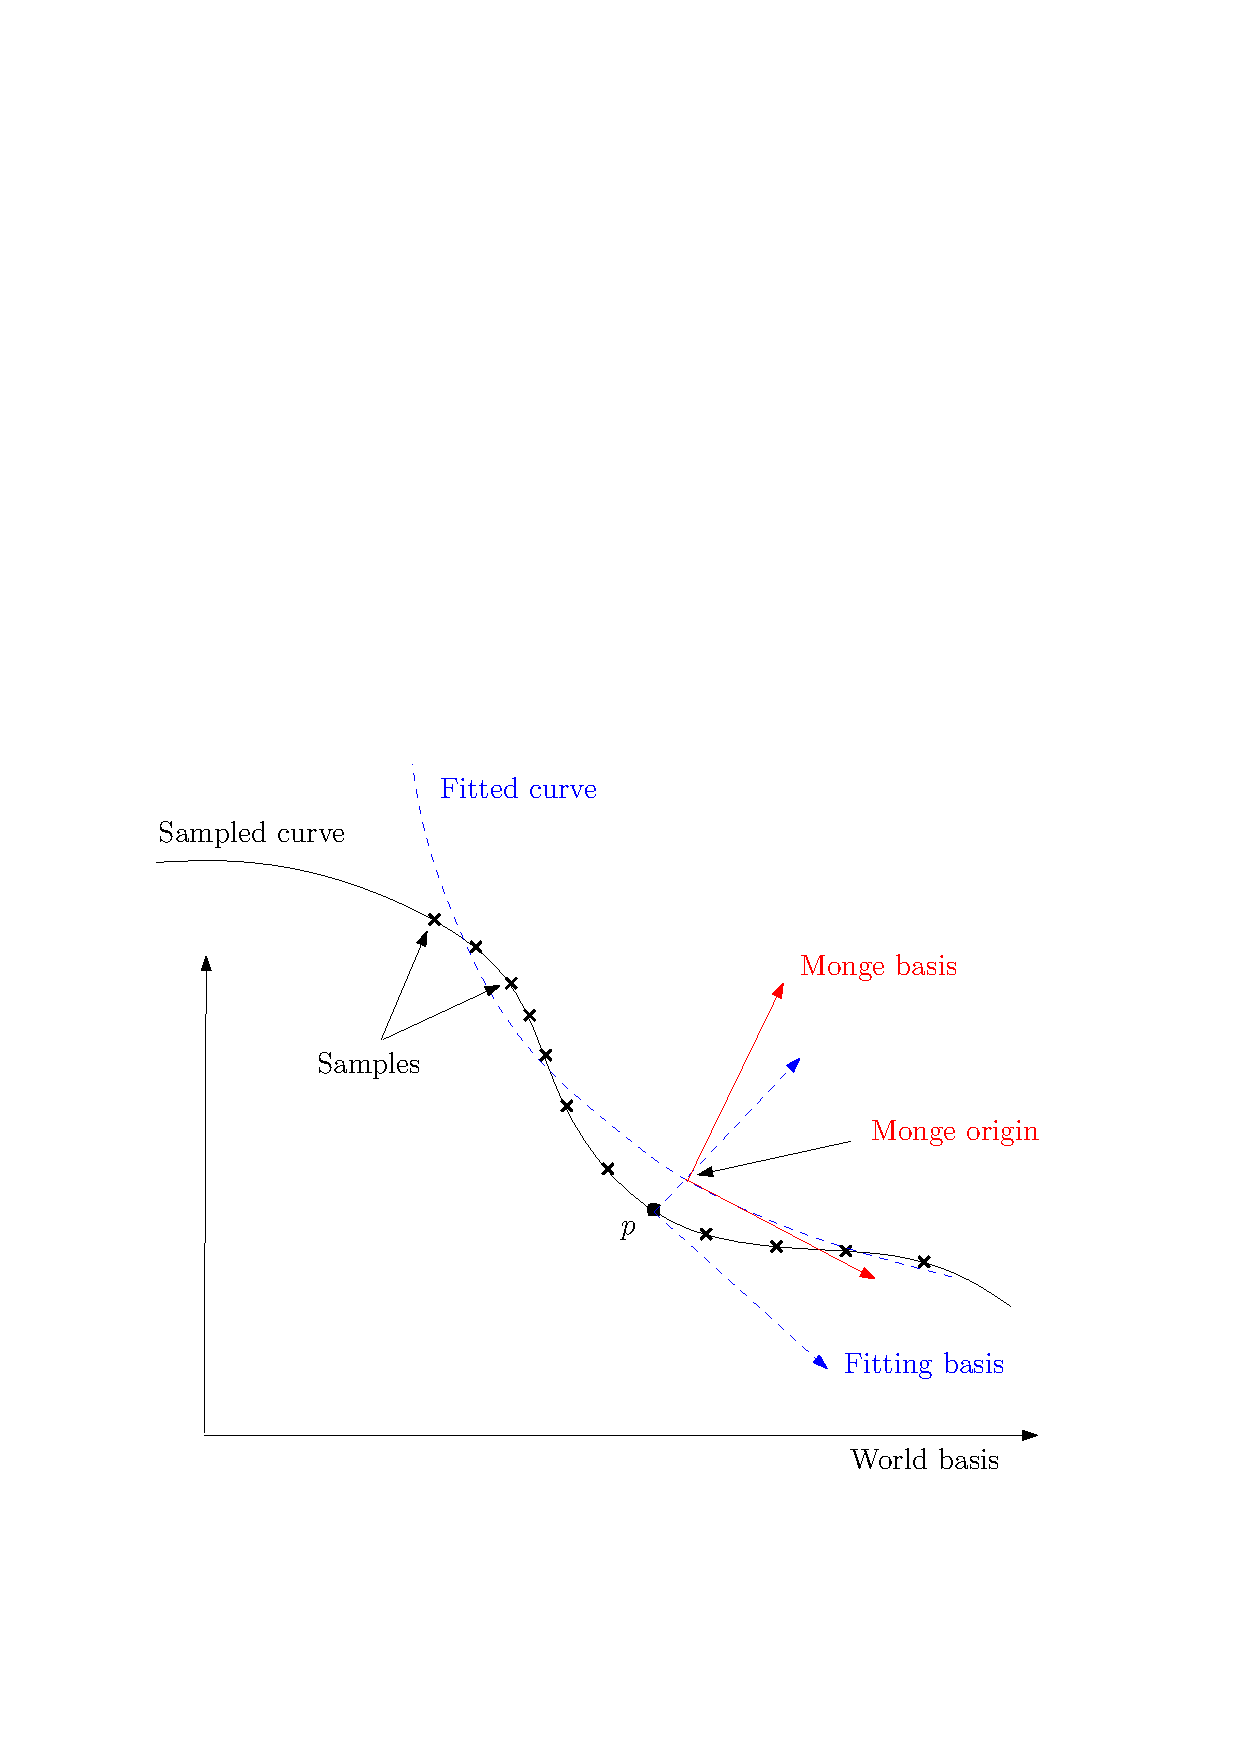
\includegraphics[width=.5\linewidth]{Jet_fitting_3/jet_fitting_basis}}
\end{ccTexOnly}

\label{fig:jet_fitting_basis}
\caption{The three basis involved in the estimation.}

\begin{ccHtmlOnly}
<CENTER>
<img border=0 src="./jet_fitting_basis.gif" width=600>
</CENTER>
\end{ccHtmlOnly}
\end{figure}

\subsection{Computing a basis for the fitting}
%%%%%%%%%%%%%%%%%%%%%%%%%%%%%%%%%%%%%%%%%%%%%%%%%%%%%%%%%%%%%

{\bf Input : samples\\ Output : fitting-basis}


%, and we
%shall assume a function {\tt eigen\_symm\_algo} doing so is available.
%
%a Principal Component Analysis, this means we need a linear
%algebra method to perform an eigen analysis of a symmetric matrix :
%{\tt eigen\_symm\_algo}. 
%
Performing a PCA requires diagonalizing a symmetric matrix.  This
analysis gives an orthonormal basis whose $z$-axis is provided by the
eigenvector associated to the smallest eigenvalue
\footnote{Another possibility is to choose as z-axis the axis of the
world-basis with the least angle with the axis determined with the
PCA. Then the change of basis reduces to a permutation of axis.}. Note
one may have to swap the orientation of a vector to get a direct
basis.

Let's note $P_{W\rightarrow F}$ the matrix to change coordinates from the
world-basis $(w_x,w_y,w_z)$ to the fitting-basis $(f_x,f_y,f_z)$. The
rows of $P_{W\rightarrow F}$ are the coordinates of the vectors
$(f_x,f_y,f_z)$ in the world-basis. This matrix represents a
orthogonal transformation hence its inverse is its transpose. To obtain
the coordinates of a point in the fitting-basis from the coordinates
in the world-basis, one has to multiply by $ P_{W\rightarrow F}$.

As mentioned above, the eigenvalues are returned, from which the
sampling quality can be assessed by checking one eigenvalue is
significantly smaller.


\paragraph{Implementation details.}
We assume a \ccc{eigen_symm_algo} function is provided by the traits
\ccc{LinAlgTraits}.
%%
This function computes the eigenvalues and eigenvectors of a real
symmetric matrix. Eigen values are sorted in ascending order, eigen
vectors are sorted in accordance.  The eigenvectors are guaranteed to
be mutually orthogonal and normalised to unit magnitude.

\subsection{Solving the interpolation / approximation problem}
\label{sec:solving}
%%%%%%%%%%%%%%%%%%%%%%%%%%%%%%%%%%%%%%%%%%%%%%%%%%%%%%%%%%%%%

{\bf Input : samples, fitting-basis \\ Output : coefficients $A_{i,j}$ of the
bivariate fitted polynomial in the fitting-basis }

Computations are done in the fitting-basis and the origin is the point
$p$. First, one has to transform coordinates of sample points with a
translation ($-p$) and multiplication by $ P_{W\rightarrow F}$.


We solve the system $MA=Z$, in the least square sense for
approximation. There is a preconditioning of the matrix $M$ so as to
improve the condition number. Assuming the $\{x_i\}$, $\{y_i\}$ are of
order $h$, the pre-conditioning consists of performing a column
scaling by dividing each monomial $x_i^ky_i^l$ by $h^{k+l}$ ---refer
to Eq. (\ref{eq:fit-linalg}). Practically, the parameter $h$ is chosen
as the mean value of the $\{x_i\}$ and $\{y_i\}$. In other words, the
new system is $M'Y=(MD^{-1}(DA)=Z$ with $D$ the diagonal matrix
$D=(1,h,h,h^2,\ldots,h^d,h^d)$, so that the solution $A$ of the
original system is $A=D^{-1}Y$.

There is always a single solution since for under constrained systems
we also minimize $||A||_2$.  The method uses a singular value
decomposition of the $N\times N_d$ matrix $M= U S V^T$, where $U$ is a
$N \times N$ orthogonal matrix, $V$ is a $N_d \times N_d$ orthogonal
matrix and $S$ is a $N\times N_d$ matrix with the singular values on
its diagonal. Denote $r$ the rank of $M$, we can decompose
%
$S= \left( \begin{array}{cc}
D_r & 0_{r,\ N_d-r}\\
0_{N-r,\ r} & 0_{N-r,\ N_d-r}
\end{array} 
\right).
$
%
The number $r$, which is the number of non zero singular values, is
strictly lower than $N_d$ if the system is under constrained. In any
case, the unique solution which minimize $||A||_2$ is given by~:
\begin{equation}
A= V
\left( \begin{array}{cc}
D_r^{-1} & 0_{N_d-r,\ r}\\
0_{r,\ N-r} & 0_{N_d-r,\ N-r}
\end{array} 
\right)
 U^TZ.
\end{equation}
%%
One can provide the condition number of the matrix $M$ (after
preconditioning) which is the ratio of the maximal and the minimal
singular values. It is infinite if the system is under constrained,
that is the smallest singular value is zero. Then, an exception is
raised.

\paragraph{Implementation details.}
We assume a \ccc{solve_ls_svd_algo} function is provided by the traits
\ccc{LinAlgTraits}. This function solves the system MX=B (in the least square sense
if M is not square) using a Singular Value Decomposition and gives the
condition number of M. 

\medskip
Remark: as an alternative, other methods may be used to solve the
system. A $QR$ decomposition can be substituted to the $SVD$. One can
also use the normal equation $M^TMX=MTB$ and apply methods for square
systems such as $LU$, $QR$ or Cholesky since $M^TM$ is symmetric
definite positive when $M$ has full rank. 
%LU suitable for any square M
%QR for rectangular
%Choleski for symm def + =LL^t
The advantages of the $SVD$
is that it works directly on the rectangular system and gives the
condition number of the system. For more on these alternatives, see
\cite{gl-mc-83}.

\subsection{Principal  curvature / directions}
%%%%%%%%%%%%%%%%%%%%%%%%%%%%%%%%%%%%%%%%%%%%%%

{\bf Input : coefficients of the fit $A_{i,j}$, 
fitting-basis \\
Output : monge-basis wrt fitting-basis and world-basis
}

In the fitting basis, we have determined a height function expressed
by Eq. (\ref{eq-answer}). Computations are done in the fitting-basis.
The partial derivatives, evaluated at $(x,y)=(0,0)$, of the fitted
polynomial $J_{A,d}(x,y)$ are
$A_{i,j}=\frac{\partial^{i+j}J_{A,d}}{\partial^ix \partial^jy}$
%%
Expanding Eq. (\ref{eq-answer}) yields:
%%
\begin{eqnarray}
J_{A,d}(x,y)&=
A_{0,0}+A_{1,0}x+A_{0,1}y+\frac{1}{2}(A_{2,0}x^2+2A_{1,1}xy+A_{0,2}y^2) 
+ \frac{1}{6}(A_{3,0}x^3+3A_{2,1}x^2y+\ldots )+ \ldots 
\end{eqnarray}


---The origin, that is the point of the fitted surface where the
estimation is performed, is $(0,0,A_{0,0})$. \\
%%
---The normal is
$n=(-A_{1,0},-A_{0,1},1)/\sqrt{A_{1,0}^2+A_{0,1}^2+1}$.\\
%%
---Curvature related properties are retrieved resorting to standard
differential calculus \cite{c-dgcs-76}. More precisely, the Weingarten
operator $W=-I^{-1}II$ is first computed in the basis of the tangent
plane $\{ (1,0,A_{1,0}), (0,1,A_{0,1}) \}$. We compute an orthonormal
basis of the tangent plane using the Gram-Schimdt algorithm, and then
we compute Weingarten in this basis (apply a change of basis matrix
$W'=P^{-1}WP$). It is then symmetric, we can apply the eigensystem
function for a symmetric matrix:
\verb+eigen_symm_algo+.
One finally gets the principal curvatures which are the eigenvalues of
$W$ and the principal directions. Sort the values and give an
orthonormal direct basis $(d_1,d_2,n)$. Let's note $P_{F
\rightarrow M}$ the matrix to change coordinates from the
fitting-basis to the monge-basis. Its rows are the coordinates of the
vectors $(d_1,d_2,n)$ in the fitting-basis. It is an orthogonal matrix
$P_{F \rightarrow M}^{-1}=P_{F \rightarrow M}^T$. The monge-basis
expressed in the world-basis is obtained by multiplying the coordinates
of $(d_1,d_2,n)$ in the fitting-basis by $P_{W\rightarrow F}^{-1}$,
(the same holds for the origin point which has in addition to be
translated by $p$, i.e. the coordinates of the origin point are
$P_{W\rightarrow F}^{-1} (0,0,A_{0,0}) +p$.

\subsection{Computing  higher order Monge coefficients}

{\bf Input : coefficients of the fit, monge-basis wrt fitting-basis ($P_{F
\rightarrow M}$)\\ 
Output : third and fourth order coefficients of Monge}

We use explicit formula. The implicit equation of the fitted
polynomial surface in the fitting-basis with origin the point
$(0,0,A_{0,0})$ is $Q=0$ with
\begin{equation}
Q=-w-A_{0,0}  +\sum_{i,j}\frac{A_{i,j}u^iv^j}{i!j!}.
\end{equation}
%%
The equation in the monge-basis is obtained by substituting $(u,v,w)$
by $P^T_{F\rightarrow M}(x,y,z)$. Denote $f(x,y,z)=0$ this implicit
equation. By definition of the monge-basis, we have locally (at
$(0,0,0)$)
\begin{equation}
f(x,y,z)=0 \Leftrightarrow z=g(x,y)
\end{equation}
and the Taylor expansion of $g$ at $(0,0)$ are the Monge coefficients
sought.
%
Let's denote the partial derivatives evaluated at the origin of $f$
and $g$ by $f_{i,j,k}=\frac{\partial^{i+j+k}f}{\partial^ix
\partial^jy \partial^kz}$ and $g_{i,j}=\frac{\partial^{i+j}g}{\partial^ix
\partial^jy}$. One has $f_{1,0,0}=f_{0,1,0}=f_{1,1,0}=0$,
$g_{0,0}=g_{1,0}=g_{0,1}=g_{1,1}=0$ and $g_{2,0}=k_1$,
$g_{0,2}=k_2$. The partial derivative of order $n$ of $f$ depends on
the matrix $P_{F\rightarrow M}$ and the partial derivatives of order
at most $n$ of $J_{A,d}$. The third and fourth order coefficients of are
computed with the implicit function theorem~:
\begin{eqnarray*}
%&b_0=g_{3,0}=-(f_{3,0,0}-3f_{1,0,1}f_{2,0,0}/f_{0,0,1})/f_{0,0,1}\\
%&b_3=g_{0,3}=-(f_{0,3,0}-3f_{0,1,1}f_{0,2,0}/f_{0,0,1})/f_{0,0,1}\\
%&c_0=g_{4,0}=-(f_{4,0,0}+3f_{2,0,1}g_{2,0}+f_{0,0,2}g_{2,0}^2
%+4f_{1,0,1}g_{30})/f_{0,0,1}\\
%&c_4=g_{0,4}=-(f_{0,4,0}+3f_{0,2,1}g_{0,2}+f_{0,0,2}g_{0,2}^2
%+4f_{0,1,1}g_{0,3})/f_{0,0,1}\\
&b_0=g_{3,0}=-{\frac { f_{3,0,0} f_{0,0,1} -3\, f_{1,0,1} f_{2,0,0} }{
f_{0,0,1} ^{2}}}
\\
&b_1=g_{2,1}=-{\frac {-  f_{0,1,1}      f_{2,0,0}    +  f_{2,1,0}    f_{0,0,1}  }{  f_{0,0,1}    ^{2}}}
\\
&b_2=g_{1,2}=-{\frac {  f_{1,2,0}    f_{0,0,1}  -  f_{1,0,1}      f_{0,2,0}    }{  f_{0,0,1}    ^{2}}}
\\
&b_3=g_{0,3}=-{\frac {  f_{0,3,0}    f_{0,0,1}  -3\,  f_{0,1,1}      f_{0,2,0}    }{  f_{0,0,1}    ^{2}}}
\\
&c_0=g_{4,0}={\frac {-3\,  f_{0,0,2}        f_{2,0,0}      ^{2}-  f_{4,0,0}      f_{0,0,1}    ^{2}+6\,  f_{2,0,1}    f_{0,0,1}    f_{2,0,0}    +4\,  f_{1,0,1}    f_{0,0,1}    f_{3,0,0}    -12\,    f_{1,0,1}      ^{2}  f_{2,0,0}    }{  f_{0,0,1}    ^{3}}}
\\
&c_1=g_{3,1}={\frac {-6\,  f_{1,0,1}      f_{0,1,1}      f_{2,0,0}    +3\,f_{0,0,1}    f_{1,1,1}      f_{2,0,0}    +3\,  f_{1,0,1}    f_{0,0,1}    f_{2,1,0}    +  f_{0,1,1}    f_{0,0,1}    f_{3,0,0}    -  f_{3,1,0}      f_{0,0,1}    ^{2}}{  f_{0,0,1}    ^{3}}}
\\
&c_2=g_{2,2}=-{\frac {  f_{2,2,0}      f_{0,0,1}    ^{2}-  f_{2,0,1}   f_{0,0,1}    f_{0,2,0}    -2\,  f_{1,0,1}    f_{0,0,1}    f_{1,2,0}    +2\,    f_{1,0,1}      ^{2}  f_{0,2,0}    -  f_{0,2,1}    f_{0,0,1}    f_{2,0,0}    +2\,    f_{0,1,1}      ^{2}  f_{2,0,0}    -2\,  f_{0,1,1}    f_{0,0,1}    f_{2,1,0}    +  f_{0,0,2}      f_{0,2,0}      f_{2,0,0}    }{  f_{0,0,1}    ^{3}}}
\\
&c_3=g_{1,3}=-{\frac {  f_{1,3,0}      f_{0,0,1}    ^{2}+6\,  f_{1,0,1}      f_{0,1,1}      f_{0,2,0}    -3\,  f_{0,1,1}    f_{0,0,1}    f_{1,2,0}    -3\,  f_{1,1,1}    f_{0,0,1}    f_{0,2,0}    -  f_{1,0,1}    f_{0,0,1}    f_{0,3,0}    }{  f_{0,0,1}    ^{3}}}
\\
&c_4=g_{0,4}=-{\frac {  f_{0,4,0}     f_{0,0,1}    ^{2}+3\,  f_{0,0,2}        f_{0,2,0}      ^{2}-6\,  f_{0,2,1}    f_{0,0,1}    f_{0,2,0}    -4\,  f_{0,1,1}    f_{0,0,1}    f_{0,3,0}    +12\,    f_{0,1,1}      ^{2}  f_{0,2,0}    }{  f_{0,0,1}    ^{3}}}
\end{eqnarray*} 

\section{Software Design}
%%%%%%%%%%%%%%%%%%%%%%%

Following \cgal's best practices in geometric software development,
the package developed in fully generic in the C++ sense ---and is
templated by three classes.

\subsection{Options and interface specifications}
%%%%%%%%%%%%%%%%%%%%%

Using the fitting strategy requires specifying two degrees: the degree
$d$ of the fitted polynomial ($d \geq 1$), and the degree $d'$ of the
monge coefficients one wants to compute, with $d' \leq d $.  In the sequel,
we also assume users are satisfied with Monge coefficients of order
four, that is, we assume $d' \leq 4$.
\medskip

Regarding interpolation versus approximation, we provide a single
function \ccc{Monge_via_jet_fitting} with parameters $d,d'$ and a
range iterator. If $N=N_d$ then interpolation is performed, else
$N > N_d$ and approximation is used. 

Preconditions are the following :

\begin{itemize}
\item
$N \geq N_d$
\item
$1 \leq d$, $d' \leq d$, $1 \leq d' \leq 4$ 
\end{itemize}	
 
\subsection{Output}
%%%%%%%%%%%%%%%%%%%%

As explained in section \ref{sec:intro}, the output consists of a
coordinate system, the Monge basis, together with the Monge
coefficients which are stored in a Monge\_rep class. In addition, more
information on the computational issues are stored in a Monge\_info
class.

The Monge basis is expressed in the world\_basis. These informations
desere the following comments.

\paragraph{Origin.} This is the point on the fitted polynomial surface
where the differential quantities have been computed. In the
approximation case, it differs from the input point $p$, it is the
point with coordinates $(0,0,A_{0,0})$ in the fitting-basis.

\paragraph{Monge basis.} The monge-basis $(d_1,d_2,n)$ is orthonormal
direct, and the maximal, minimal curvatures are defined wrt this
basis. If the user has a predefined normal $n_0$ (e.g. the sample
points come from an oriented mesh) then if $n_0 . n >0$ then max-min is
correct, if $n_0 . n <0$ then the user should prefer the orthonormal
direct basis $(d_1',d_2',n')=(d_2,d_1,-n)$ with the maximal curvature
$k_1'=-k_2$ and the minimal curvature $k_2'=-k_1$. If $n_0 . n =0$ or
is small then this means that the orientation of the surface is not so
clear!

\paragraph{Monge coefficients.}
The vector of coefficient of the Monge form is $(k_1, k_2 (\leq k_1),
b_0, b_1, b_2, b_3, c_0, c_1, c_2, c_3, c_4)$ for $d' = 4$.

\subsection{Template parameters}
%%%%%%%%%%%%%%%%%%%%%%%%%%%%%%%%%

The following picture illustrates the template dependencies.
\begin{figure}[h!]
\begin{ccTexOnly}
\centerline{
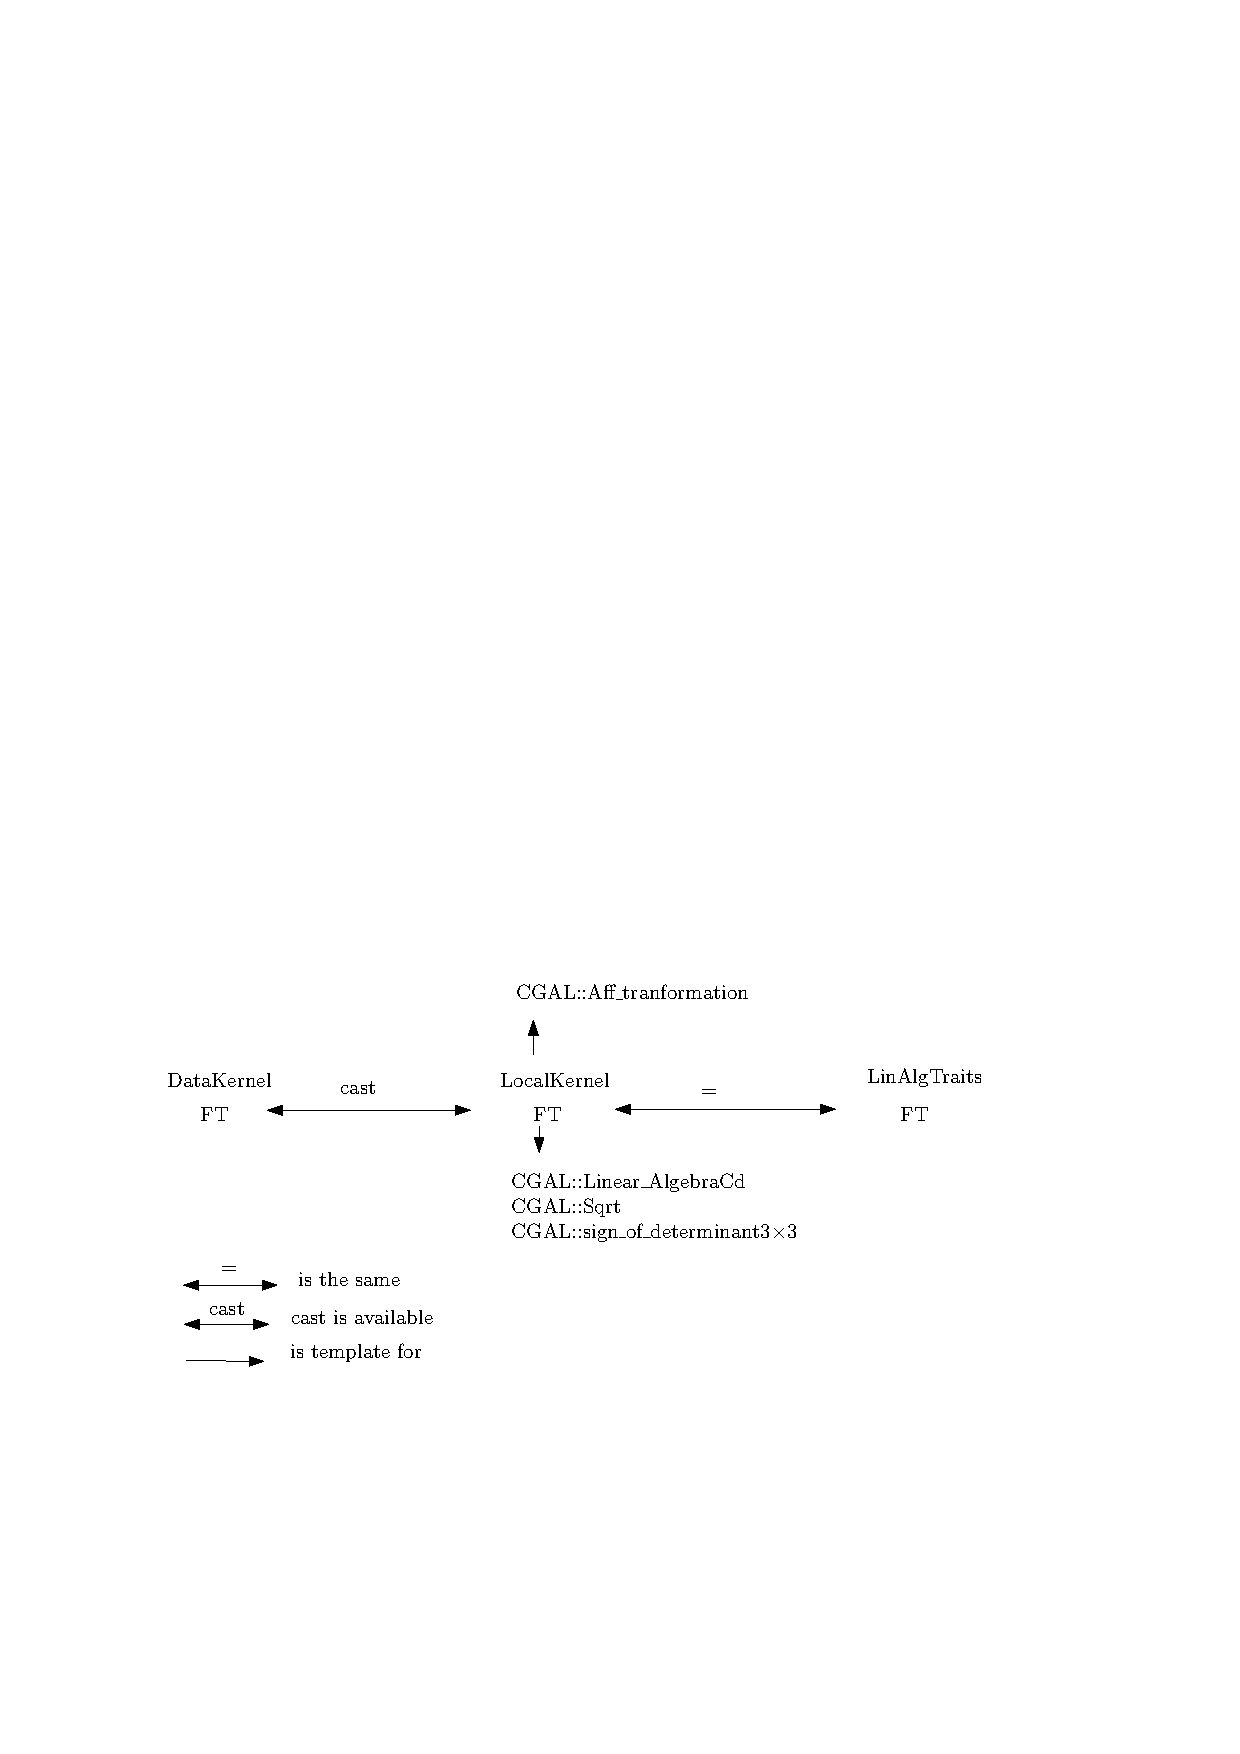
\includegraphics[width=.5\linewidth]{Jet_fitting_3_ref/template_dependence}}
\end{ccTexOnly}

%\label{fig:template_dependence}
%\caption{}

\begin{ccHtmlOnly}
<CENTER>
<img border=0 src="template_dependence.jpg" width=600>
</CENTER>
\end{ccHtmlOnly}
\end{figure}

More details are given in the reference manual.

\subsubsection{Template class \ccc{Data_Kernel}}
%%%%%%%%%%%

This class provides the types for the input sample points, together
with $3d$ vectors and a number type. It is used as template for the
\ccc{Monge_rep}. Typically, one can use \ccc{CGAL::Cartesian<double>}.

\subsubsection{Template class \ccc{Local_Kernel}}
%%%%%%%%%%%

This class defines the vector and number types used (i)\ for local
computations (ii)\ to store the Monge\_info class members. Input
points of type \ccc{Data_Kernel::Point_3} are converted to
\ccc{Local_Kernel::Point_3}. For output of the \ccc{Monge_rep} class, these
types are converted back to \ccc{Data_Kernel} ones.  Typically, one can use
\ccc{CGAL::Cartesian<double>}.

\subsubsection{Template class \ccc{Linalg_traits.}}
%%%%%%%%%%%

This class provides the matrix algebra operations required by the
fitting method. These are an eigen method for symmetric mtrices and
linear solver using a singular value decomposition.

\subsubsection{Compatibility requirements}

An important requirement is the following. To solve the fitting
problem, the coordinates of the samples undergo two types of
operations: first, an eigen analysis is performed in the world-basis
(with the LinAlgTraits::FT which is also the LocalKernel::FT); second,
points are expressed into fitting-basis; third, matrices used for the
linear algebra operations are filled from powers of the coordinates of
the samples in fitting-basis. Linear algebra operations being used for
these three stages, we assume the linear algebra traits class provides
functions compatible with the number type defining the coordinates of
the samples. In particular, for number types supporting
multi-precision, this requires converting the samples into points with
more standard types ---unless the user has a package supporting linear
algebra operation on such number types.





\section{Examples} 
%%%%%%%%%%%%%%%%%%%%%%%%%%%%%%%%%%%%%%%%%%%%%%%%%%%%%%%%%%%%%%%%%%%%%%%%%%%%

\paragraph{About a point.}
The first example illustrates the computation of the local
differential quantities from a set of points given in a text file as
input. The first point of the list is the one at which the computation
is performed. The user has to specify a file for the input points, a
file to output the results, the degrees $d$ and $d'$.
\ccIncludeExampleCode{Jet_fitting_3/blind_1pt.C}

\paragraph{On a mesh.}
The second example (cf blind.C in the exemple directory) illustrates
the computation of local differential quantities for all vertices of a
given mesh. Results are twofold:
\begin{itemize}
\item
a human readable text file featuring the Monge\_rep and the Monge\_info data;
\item
another text file which may be visualised with the demo program
visu.exe displaying the Monge basis at each vertex of the mesh.
\end{itemize}

%\ccIncludeExampleCode{Jet_fitting_3/blind.C} %too long to be included?
